 \documentclass[12pt,a4paper]{article}
\usepackage[utf8]{inputenc}
\usepackage{amsmath}
\usepackage{amsfonts}
\usepackage{amssymb}
\usepackage{gensymb}
\usepackage{graphicx} %package to manage images
\graphicspath{ {./images/} }
\usepackage[hide]{chato-notes}
\newcommand{\ceg}[1]{\mynote[author=EG]{#1}}
\newcommand{\cvt}[1]{\reply[author=VT]{#1}}
\author{Viet Ta}
\title{Redescription Mining from Boolean data with a hierarchy}
\begin{document}
\maketitle

\ceg{You should add a few citations to related work, when you introduce the problem, etc.}
\cvt{Done}
\ceg{Where?}
\cvt{fixed}
With the enormous amount of data we produce nowadays, data mining is becoming more and more prevalent. Consequently, the modern idea of data mining is not only to discover information from crude data, but also to condense that information down to concise descriptions and insights. One method of such ``insights mining'' is redescription mining \cite{DBLP:journals/corr/cs-CE-0311048}. In a nutshell, redescription mining is to find two different ways to describe the same thing.

\ceg{Start with the input description, (i.e. describing the input to the problem) on a more concrete level (but general not limited to one very specific instance), i.e.\ not tuple of sets and maths symbols. Rather simply, we have a collection of objects, also called entities, and variables, also called attributes, and the data contains the values of the attributes for each of the objects collected in a table. etc. You can start the example there. Then, you can explain what the aim of redescription mining is in this context.}
\cvt{Done}
\ceg{You need to proceed more clearly in \textbf{stages} from generic bio-climatic niche finding to specific example query. You need to explain what the task of bio-climatic niche finding consists in (and why it is useful),  i.e. characterize the habitat of species in terms of the climatic conditions, then how it is cast into the redescription mining framework given the data (what are the entities, the variables, the two views?) look for pairs of queries, one selecting one or a few species, the other selecting a few climate variable and associated restrictions to value range, then provide a particular example}
\cvt{Done}
\ceg{The "many applications" sounds actually quite restrictive since it only mentions (paleo)ecology. Also redescription mining does not aim to forecast anything, it helps to study patterns which might then allow to make predictions.}
\cvt{Fixed}

Redescription mining can be applied in many fields, e.g. biology, ecology, social and political science, engineering, etc \cite{galbrun2018redescription}.
One classic example of redescription mining is about finding bio-climatic niche \cite{10.2307/4072271}. 
In this example, we want to find the bio-climatic niche by drawing out the relation between the geographical distribution data of species and geographical climate data.
\ceg{This simplifies "finding bioclimatic niches" (we don't actually know what this means) to highlighting the relation between max march temperature and Lynx species. This does not work.}
\cvt{Fixed}
\begin{figure}[t]
 \centering
 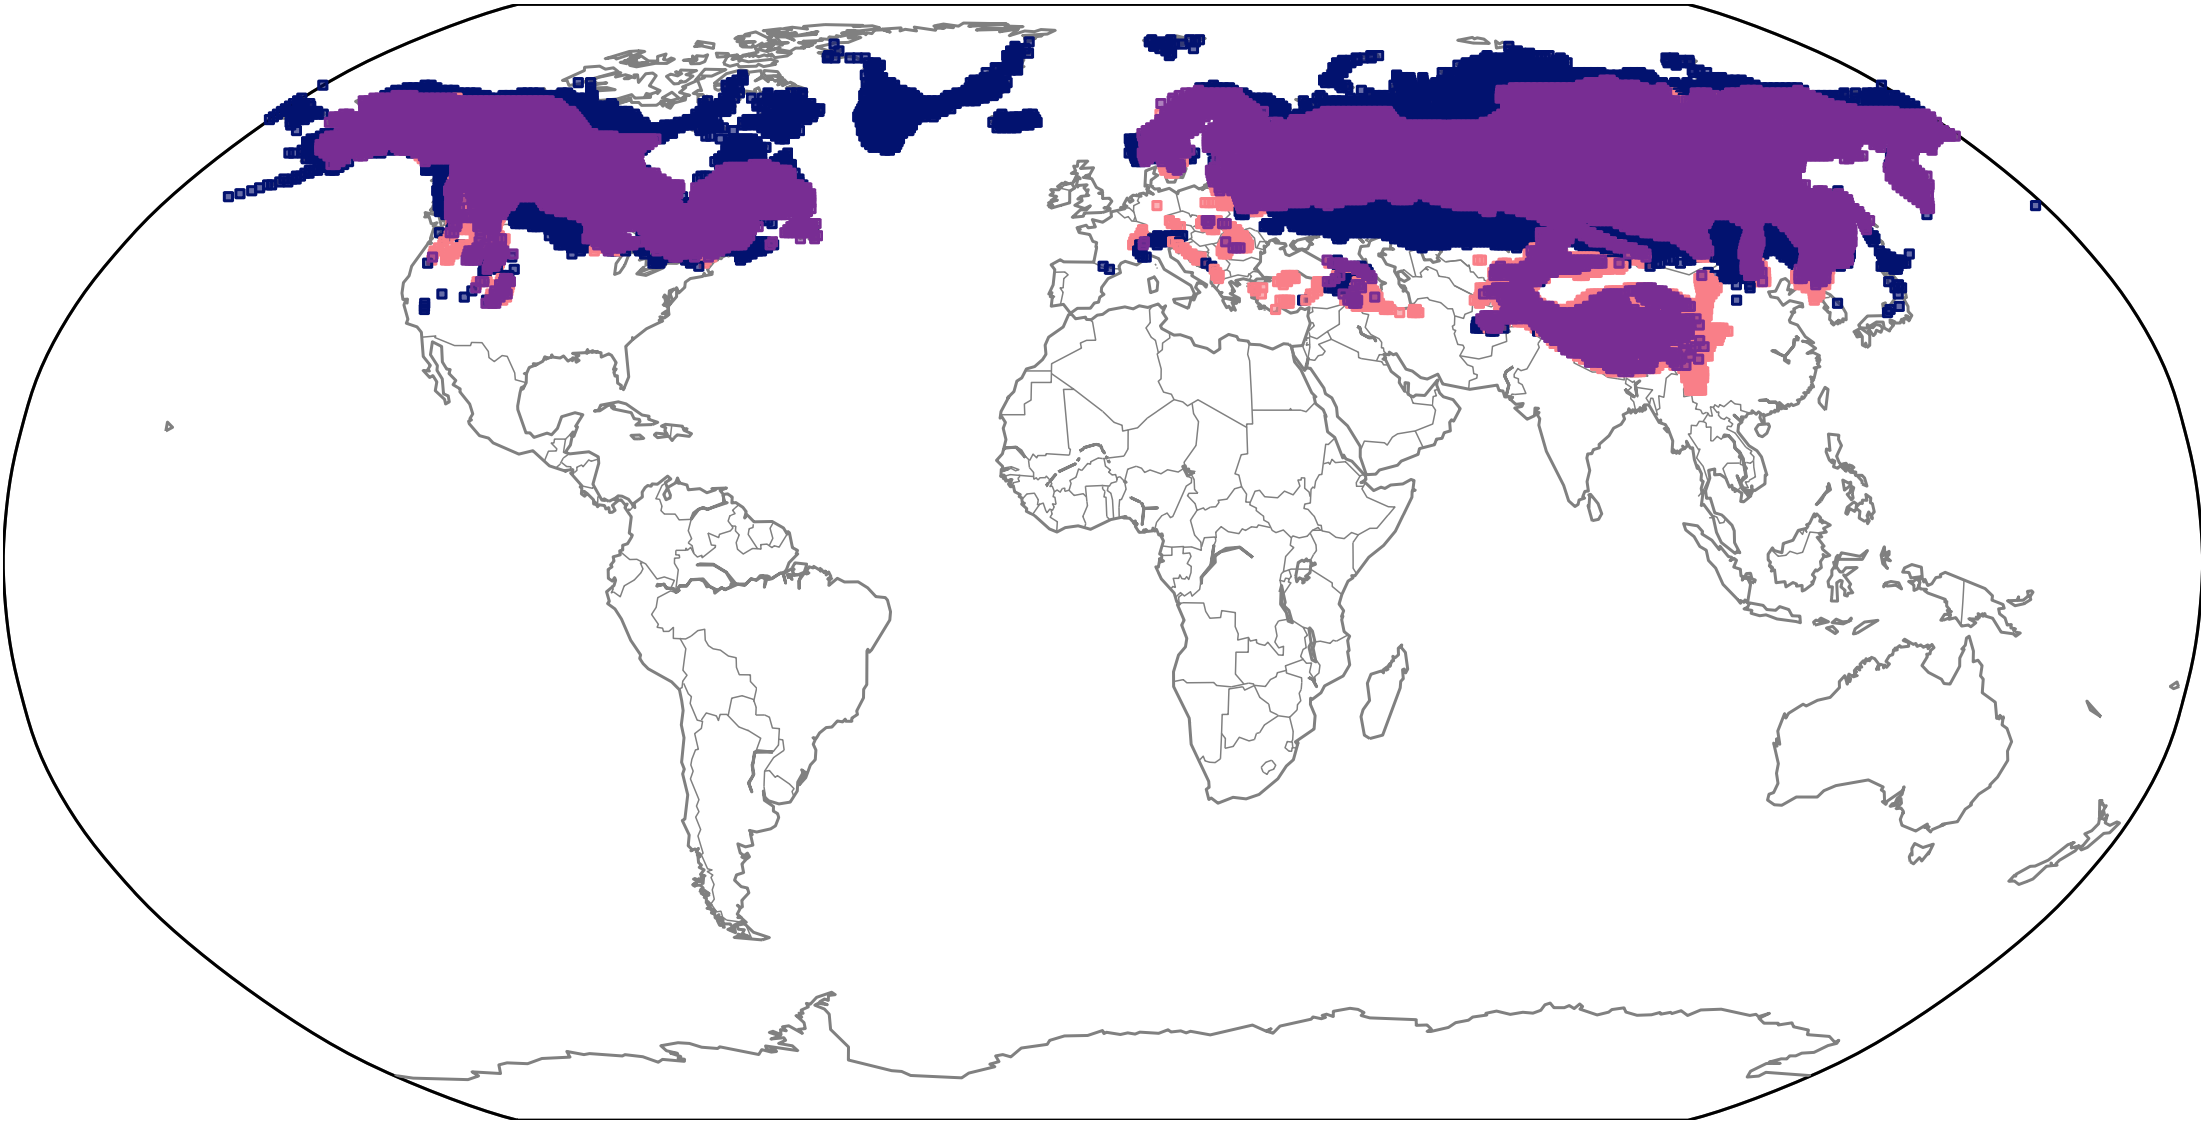
\includegraphics[width=10cm]{niche-finding}
 \caption{The areas inhabited by lynxes (light red and medium purple) and the areas where the maximum March temperature is between $-24.4 \degree C$ and $3.4\degree C$ (dark blue and medium purple) \cite{galbrun2018redescription}}
 \label{fig:niche}
\end{figure}
For example, the technique can find out that the area where maximum March temperature in a specific range is relatively similar to the area where some mammals, e.g. lynxes, are distributed, see figure \ref{fig:niche}.
Here the first description is about the maximum March temperature range, and the second description is about the distribution of lynxes. \ceg{what are the descriptions and what is being described?} \cvt{Did I fix this?}
Both the descriptions and what they describe in this case carry useful information. For instance, an ecologist might look at the descriptions to understand the model of the niche, and the geographical data for the niche areas.
\ceg{explain what the data is in terms introduced before, esp. pointing out what the two views are}
\cvt{Done}

Intuitively, the redescription mining model is analogous to the concept of data table, i.e. there is a pair of tables which mapped through the rows, each one contains data for one view. \ceg{one table contains the data from one view, so with two views, we have a pair of tables (mapped through the rows)}\cvt{fixed} Entities are represented as rows, attributes correspond to columns, one view is just set of column(s). The data is essentially the values of the attributes collected in a table. All the rows those satisfy the criteria of a query are called the support (or support set) of that query. Formalizing the previous example, the geographical regions are called entities (a.k.a objects), while species inhabiting the regions and temperature variables are the attributes of those entities, a set of attributes is a view, see table \ref{tab:mammals-and-climate}.
Our goal here is to find two different queries, one over each view, where the supports of them are sufficiently overlapped. \ceg{two queries, one over each of the view. What does that mean to "have similar results"?}\cvt{fixed} Such pair of queries is called a redescription.

\begin{table}[]
\resizebox{\textwidth}{!}{%
\begin{tabular}{|l|l|l|l|l|l|l|l|l|l|l|}
\cline{1-5} \cline{7-11}
\multicolumn{5}{|c|}{Mammals distribution data} &  & \multicolumn{5}{c|}{Climate Data}                                  \\ \cline{1-5} \cline{7-11} 
Location ID   & ...   & Lynx   & Rabbit  & ...  &  & Location ID & ... & Max March Temperature ($\degree C$) & Rain Fall in May ($mm$) & ... \\ \cline{1-5} \cline{7-11} 
...  & ... & ...   & ...  & ... &  & ...  & ... & ... & ... & ... \\ \cline{1-5} \cline{7-11} 
4652 & ... & True  & True & ... &  & 1234 & ... & 5   & 10  & ... \\ \cline{1-5} \cline{7-11} 
4653 & ... & False & True & ... &  & 5678 & ... & 8   & 40  & ... \\ \cline{1-5} \cline{7-11} 
.... & ... & ...   & ...  & ... &  & .... & ... & ... & ... & ... \\ \cline{1-5} \cline{7-11} 
\end{tabular}%
}
\caption{Mammals and climate data on two row mapped tables}
\label{tab:mammals-and-climate}
\end{table}
 
The formal definition of redescription mining was described in \cite{Galbrun-Methods}, where the data model is a tuple of 3 sets: $entities$, $attributes$, and $views$. Each entity is associated with a set of $attributes$. The $attributes$ are partitioned into disjoint $views$. Then, a description is simply a query evaluates each entity and output a Boolean value. And finally, a support of a query is a set of entities in the data that renders true in the query.
\ceg{you need to connect the formal definition and the example}
A redescription is a pair of descriptions with disjoint views and sufficiently similar supports \cite{galbrun2018redescription}.
The similarity of two supports can be measured by a distance function. If the similarity is above a threshold then the two descriptions form a redescription.


If we keep going deeper from here, redescription mining can be branched out by the ways we define the data structure, special constrains, etc. Each one has it own algorithms and techniques, redescription mining of Boolean data with a hierarchy between the attributes is one of them.
\ceg{basically, the idea is that different types of data and of queries considered require their own algorithms, one is Boolean data with a hierarchy between the attributes}
\cvt{Done}
\ceg{Boolean data don't require discretization, depending on the type of queries considered, they might afford exhaustive search rather than a heuristic.}
\cvt{Done}
Boolean data structure is a special case of categorical data structure, where there are only two possible values of either $True$ or $False$. \ceg{need to talk about the hierarchy too}\cvt{Done}
Hierarchy is the logical arrangement the data into different levels, which can be visualized by pyramid or tree diagrams.

\ceg{try to not go back and forth between the different levels, i.e. the high level idea of what the hierarchy is and can be used, the technical aspects of how it is represented and manipulated, the specific example}
\cvt{Done}


% what's special about Boolean data algorithms?
The problem of Boolean data with a hierarchy is an interesting scenario where an additional dimension of data structure is introduced. We can add hierarchical constrain(s) to the queries, or utilize that extra information to optimize the algorithm, etc. \ceg{what can be done with it}\cvt{done?}  Also Boolean data don't require discretization, so depending on the type of queries considered, we might be able to perform an exhaustive search rather than a heuristic one.

The hierarchical information can be stored separately in a different table or even embedded into the attributes names, e.g. by prefixing, themselves. 
In the bio-climatic niche finding, \ceg{maybe more general, of a species at a location, it's clearest if you earlier explained what the data consists of, i.e.\ what are entities and variables}\cvt{Done?}the $attributes$ (e.g. presence of a species at a location) can be represented by a Boolean value: $True$ (present), or $False$ (not present). The taxonomies of biological classifications\ceg{it's actually a multi-level hierarchy, with "order", "class", "family", "sub-family", etc. Maybe give example for the lynx to make things more concrete}\cvt{Done} can be implanted to add the hierarchy to the data. For example we can prefix species names by their families: `
Lynx-Eurasian' and `Lynx-Canada'. \ceg{the wording "implanted to add the hierarchy to the data is awkward, but the idea is right}
\cvt{Do I need to change it?}
% how it affect the algorithms

The introduced hierarchical information can be exploited to prune candidates more efficiently during the mining process. For instance, if we find out that the parent does not satisfy the query, then we can automatically rule out its children from the search space. Another exploitation of the hierarchy is to put the constrains to the attributes appearing in the query, e.g. instead of having the Eurasian-lynx and Canada-lynx attributes exist independently, we can force them into one category by their family information, i.e. Lynx.  \ceg{a bit more insight maybe on why and how this is? e.g.\ related to frequency of child attribute compared to parent. Also other way in which the hierarchy can be exploited, e.g. constraints on the attributes appearing in the query} \cvt{Fixed}

\bibliographystyle{apalike}
\bibliography{references}
\end{document}